
\chapter{引言}


\section{研究背景}

随着软件产业的发展,越来越多的软件被开发出来,并在各种各样的终端设备和服务器上面得到使用,可以说,软件在我们的生活中已经随处可见。然而,伴随着各种各样软件的普及,人们不再只是对软件的功能有需求,人们逐渐对软件的性能提出了要求,毕竟在现在这个信息社会,高性能意味着用更短的时间完成工作,这样才能在有限的时间内创造出更大的价值。

在软件工程领域中,针对软件性能的管理已经存在了一些比较成熟的理论和操作方式。一些比较大型的信息技术(IT)公司都有一套比较完整和严格的性能管理和测试流程以及对应的系统,一般在这样的流程中,代码的提交和审阅都比较严格。但是这样的流程和系统一般都是适用于开发者范围比较小的软件上面使用。

\begin{figure}[H]
\centering
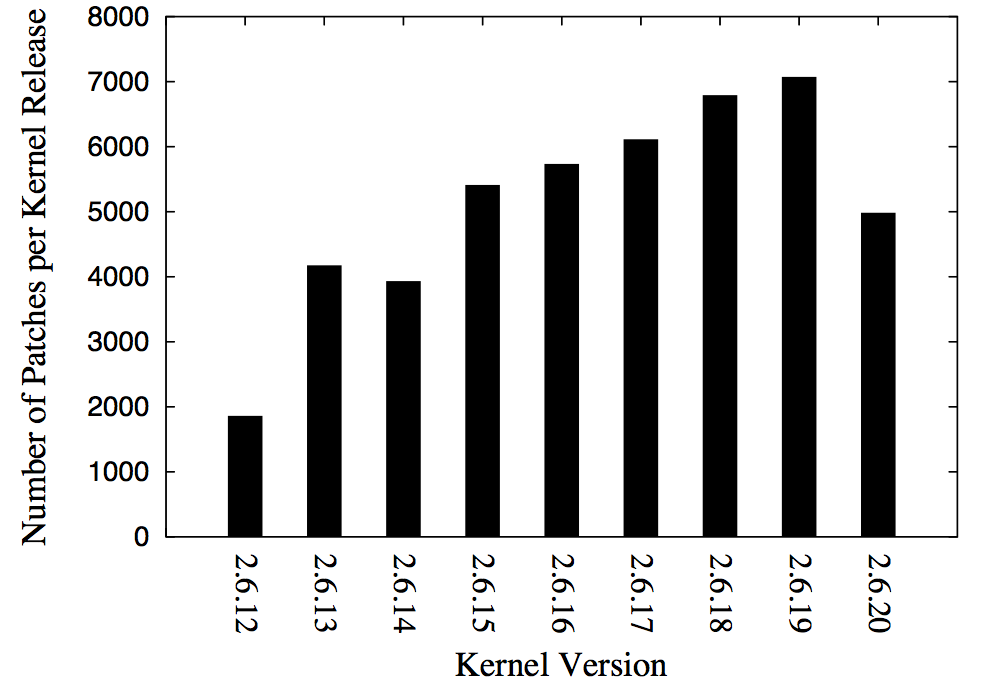
\includegraphics[width=10cm]{pactches_count}
\caption{每个Linux版本的补丁数量}
\label{fig:patches_count}
\end{figure}

Linux内核作为一款开源的操作系统(OS)内核,其开发的开放性是其他的软件无可比拟的,成千上万的开发者几乎遍布全球各地。每一个版本的Linux内核推出往往仅需要短短的几个月时间,但即使是仅仅几个月的时间,开发者们也往往为Linux内核提供了大量的代码,图\ref{fig:patches_count}\cite{chen2007keeping}记录的就是2.6.12版本到2.6.20(包含)内所有版本内纳入的开发者提交的补丁的数量。

虽然,Linux内核接受补丁的要求一般比较高,但是还是很难排除掉代码中存在的所有问题。为了方便理解,下面介绍一下Linux的开发模式。


\subsection{Linux的开发模式}

一般Linux内核的开发是分为不同的子系统分开进行的,比如内存管理(MM)和网络子系统等。
\begin{figure}[H]
\centering
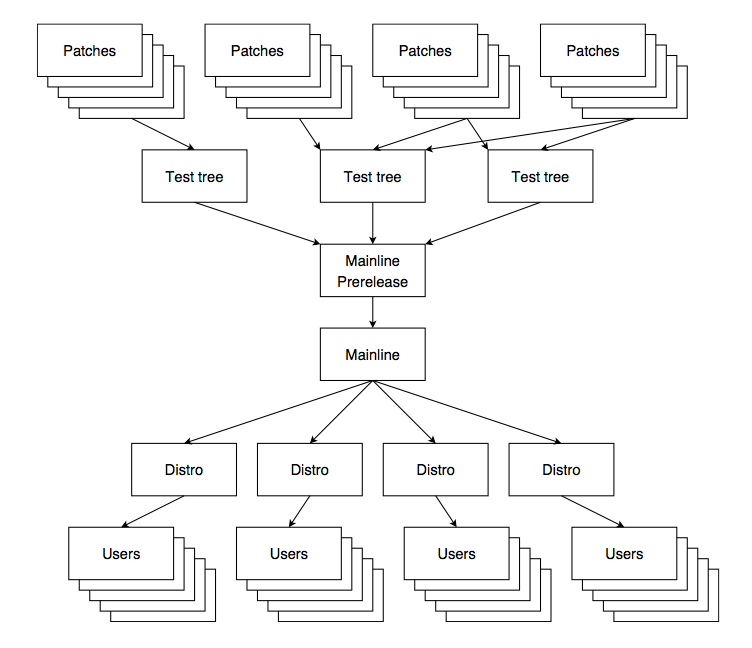
\includegraphics[width=10cm]{linux_kernel_change_flow}
\caption{Linux内核开发模式}
\label{fig:linux_kernel_change_flow}
\end{figure}

如图\ref{fig:linux_kernel_change_flow}所示,每一个子系统都会有一个单独的代码树(tree)进行比较独立的开发,并且每隔一段时间就会从主线代码树同步。

每一个内核的开发者在编写好了代码之后,生成好补丁,将补丁发送给对应子系统的代码树的管理员,管理员经过审阅之后会将补丁打在这个子系统的代码树中进行测试,一旦测试通过,在新功能的合并窗口内会被提交到主线代码树中进行进一步的测试。在一个稳定版的Linux内核正式发布之前,一般都会发布多个发行测试版,在这期间,Linux内核仅仅是对已有的功能进行修复和测试,并不添加新的功能。

在稳定版的Linux内核发布之后,各个Linux发行版厂商可以根据需要选择是否使用新版本Linux内核作为发行版的内核。

\subsection{Linux的开发特点}

随着Linux内核开发的全球化,Linux开发的步伐也逐渐加快,开发的规模也逐渐扩大,目前内核开发大致具有以下的特点:

\begin{enumerate}
\item 越来越多的新功能被添加到内核中来,导致内核的结构越来越复杂
\item 内核的复杂结构使得任何一点改动对内核性能造成影响的可能性加大
\item Linux内核进行官方测试的间隔一般比较大(一般只在有新版本发布的时候才会进行比较完整的测试)
\item 一旦发现版内核中出现性能回退的问题,这个问题就会随着各大Linux发行版扩散到广大的用户当中
\end{enumerate}

\section{课题目标}

正如研究背景所述,目前Linux内核的开发具有比较鲜明的特点,而且Linux作为一个操作系统内核,也具有一点的特殊性,因此,很有必要设计并实现出一套与Linux内核相适应的性能测试框架,方便Linux的开发者们更加方便地进行性能回退问题的管理和处理。

本课题的目的就是设计并实现一套能够进行Linux性能测试并具有如下特征的框架:

\begin{enumerate}
\item 较快并准确进行Linux性能测试
\item 在出现性能回退之后,多次运行进行问题确认
\item 确认性能回退之后,能够最快地定位到出现问题的代码
\item 在定位到问题代码之后,将相关的测试数据及出现问题的代码通知给相关代码的作者
\end{enumerate}